\documentclass[numbers=noenddot,12pt,a4paper]{scrartcl}
\usepackage[greek,ngerman]{babel}
\usepackage[T1]{fontenc}
\usepackage[utf8]{inputenc}
\usepackage{fullpage}
\usepackage{libertine}
\usepackage{ziffer}
\usepackage{graphicx}
\usepackage{units}
\usepackage[infoshow]{tabularx}
\usepackage{amsmath}
\usepackage{amssymb}
\usepackage{wrapfig}
\usepackage{esint}
\usepackage{float}
\usepackage{wrapfig}
\usepackage[font=small]{caption}
\usepackage{subcaption}
\usepackage{lscape}
\usepackage{hyperref}

\renewcommand{\thefigure}{Abb. \arabic{figure}}

\captionsetup[wrapfigure]{name=}
\captionsetup[figure]{name=}
\newcommand{\nummat}[1]{\left[\text{#1}\right]}
\newcommand{\num}[1]{$\left[\text{#1}\right]$}
\newcommand{\degree}{^\circ}
\newcommand{\diff}{\textnormal{d}}
\newcommand{\tenpo}[1]{\cdot 10^{#1}}
\newcommand{\greek}[1]{\greektext#1\latintext}
\newcommand{\ix}[1]{_\text{#1}}
\newcommand{\imag}{\mathbf{i}}
\newcommand{\tilt}[1]{\textit{#1}}
\newcommand{\grad}[1]{\textit{grad}\left(#1\right)}
\newcommand{\divergenz}[1]{\textit{div}\left(#1\right)}
\newcommand{\euler}{\mathnormal{e}}
\newcommand{\fett}[1]{\textbf{#1}}

\title{Protokoll: Optisches Pumpen} %TODO Name des Versuchs eintragen
\author{Philipp Hacker} %TODO Protokollschreiber unterstreichen
\date{\today}

\begin{document}
%\setcounter{page}{2}
%\setcounter{section}{1}
\maketitle
\begin{center}
Betreuer: G. Marx\\ %TODO Name des Betreuers eintragen
Versuchsdatum: 14.01.2015\\ %TODO Datum des Versuchs eintragen
\begin{table}[h]
\centering
Note: %TODO Gute Note erhalten :)
\begin{tabularx}{1.5cm}{|X|}
\hline \\ \\
\hline
\end{tabularx}
\end{table}
\end{center}
\vspace*{\fill}
\tableofcontents
\vfill
\newpage
\section{Einleitung}
\section{Grundlagen}
\subsection{Emission und Besetzungsinversion}\label{subsec:besetzinv}
Ein Medium, welches elektromagnetischer Strahlung ausgesetzt ist, kann Photonen bestimmter Energien aufnehmen und abgeben. Diese Vorgänge heißen Absorption und Emission. Im ersten Fall ist es so, dass die Energie eines Teilchens (Elektronen oder Nukleonen) zum Übergang von einem energetisch niedrigeren in einen höheren Zustand gerade durch ein Photon gestellt wird. Der Vorgang der Emission kann sich auf zwei Arten vollziehen. Einerseits kann ein angeregtes Teilchen, unter der Abgabe der Energiedifferenz der Niveaus in Form eines Photons, in seinen Ausgangszustand zurück relaxieren. Andererseits kann durch das äußere Strahlungsfeld ein Teilchen zur Verringerung seiner Energie induziert werden. Diese entspricht gerade der des stimulierenden Photons. Das Ergebnis der stimulierten Emission sind somit 2 Photonen gleicher Energien.\\
Ist die Änderung der Zustandsverteilungen $N\ix{i}(t)$ proportional zur ursprünglichen Anzahl $N\ix{i}(t\ix{0})$ und der Energiedichte des Strahlungsfeldes $\rho\ix{ext}$, so lässt sich für alle drei Vorgänge zwischen den Niveaus $i$ und $j$ schreiben
\begin{align}
	\text{Absorption :} \,\, \frac{\diff N\ix{i}(t)}{\diff t}=&-B\ix{ij}\cdot N\ix{i}(t\ix{0})\cdot \rho\ix{ext} \label{eq:absorp}\\
	\text{Emission :} \,\, \frac{\diff N\ix{j}(t)}{\diff t}=&\frac{\diff N\ix{j, spo.}}{\diff t}+\frac{\diff N\ix{j, stim.}}{\diff t}=\left(-B\ix{ji}\cdot \rho\ix{ext}+-A\ix{ji}\right)\cdot N\ix{j}(t\ix{0}) \label{eq:emiss} \,\,.
\end{align}
($B\ix{ij}$, $A\ix{ij}$ - Einsteinkoeffizienten des Übergangs $i\rightarrow j$) \\
Man sieht an Gl. (\ref{eq:emiss}) sofort, das die spontane Emission einem Zerfallsgesetzt mit der Halbwertszeit $\tau=1/A\ix{ji}$ entspricht.\\
Folgen die Besetzungszahlen der diskreter Energieniveaus, welche an Absorption/Emission beteiligt sind, einer statistischen Temperaturverteilung\\ (\tilt{Boltzmann-Statistik}, \tilt{Fermi-Dirac-Statistik}), so besteht eine Besetzungsinversion, wenn die Verhältnisse der Teilchenzahlen in den jeweiligen Zuständen gerade umgekehrt bezüglich der gewählten Verteilung sind.\\
Sei $E\ix{2}$ mit dem statistischen Gewicht $g\ix{2}$ ein energetisch höheres Niveau als $E\ix{1}$ mit $g\ix{1}$, so folgt für die Gleichverteilung mit der Boltzmann-Statistik bei der Temperatur $T$ die Dichte der Teilchen im Zustand $E\ix{2}$ (analog $E\ix{1}$)
\begin{align}
	N\ix{2}=&N\ix{1}\cdot\frac{g\ix{2}}{g\ix{1}}\cdot\euler^{-\frac{E\ix{2}-E\ix{1}}{k\ix{B}T}} \,. \label{eq:dichte} \\
	\text{Inversion für :} \,\, N\ix{2}>&\frac{g\ix{2}}{g\ix{1}}\cdot N\ix{1} \label{eq:invers}
	\end{align}
Wie bereits angesprochen (in \ref{subsec:fklaser} ) kann eine Besetzungsinversion ohne äußere Erregung nicht realisiert werden, wie Gl. (\ref{eq:dichte}) und (\ref{eq:invers}) mit $E\ix{2}-E\ix{1}>0$ verdeutlicht. Das heißt, dass ausgewählte, höhere Niveaus durch sogenanntes Pumpen (siehe \ref{subsec:optpump}) mit diskreten Energien des Erregungsspektrums stärker besetzt werden können. Man muss jedoch beachten, dass ein sehr kleines Frequenzband ($\delta\nu\approx\unit[10]{Hz}$) zur Anregung eines Zustandes zuständig ist. Dies ist Folge der Unschärfe des Impulses der Pump-Photonen (Gl. (\ref{eq:breite}) nach \tilt{Heisenberg}, 1927) und der Doppler-Verbreiterung (Gl. (\ref{eq:doppler}) nach \tilt{Doppler}, 1842).
\begin{align}
	2\pi\delta\nu=\frac{1}{\tau}=A\ix{ji} \label{eq:breite}\\
	\delta\nu=\frac{\overline{\nu}}{c}\sqrt{\frac{8k\ix{B}T\ln\left(2\right)}{m}} \label{eq:doppler}
\end{align}
\subsection{Optisches Pumpen}\label{subsec:optpump}
\begin{wrapfigure}[15]{ro}{0.45\textwidth}
	\vspace{-0.75cm}
	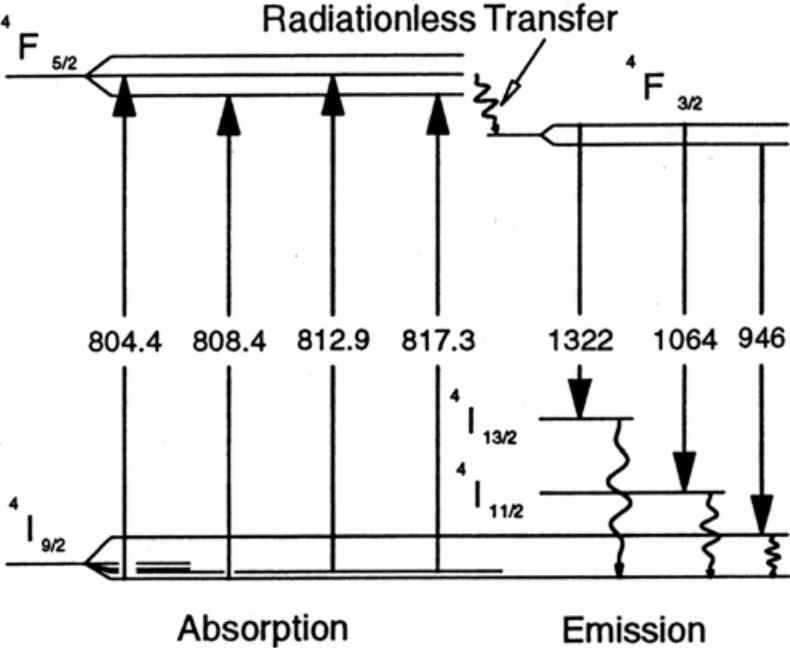
\includegraphics[width=0.45\textwidth]{uebergaenge.png}
	\caption{Termschema mit strahlungsloser Relaxation (\tilt{Radiationless Transfer}) des Nd:YAG}\label{img:übergänge}
\end{wrapfigure}
Licht, welches auf ein Medium abgestrahlt wird, ruft eine Anregung hervor und verändert damit die Besetzungen der Zustände, welche mit der Energie der Photonen korrespondieren. Die Absorption (siehe \ref{subsec:besetzinv}) der Teilchen findet nur bei diskreten Frequenzen bzw. Wellenlängen auf den atomaren Energieniveaus der Elektronen der Hülle statt, da die Photonen nur bestimmte Energien $E=\hbar\omega\,$ transportieren. Optisches Pumpen ist somit das Verfahren der spektralen Anregung eines diesbezüglich aktiven Mediums unter Ausnutzung der Besetzungen der Zustände (nach \tilt{Boltzmann}) und der Eigenschaften der Elektronen in den Hüllen. \ref{img:übergänge} zeigt die Übergänge in den Zuständen des Nd:YAG für die jeweiligen Wellenlängen.
\section{Durchführung}
\section{Auswertung}
\section{Quellen}
\end{document}